\documentclass[a4paper]{article}
\usepackage[dutch]{babel}
\usepackage{microtype}
\usepackage{url}
\usepackage[T1]{fontenc}
\usepackage{lmodern}
\usepackage{hologo}
\usepackage{graphicx}

\setlength{\voffset}{0pt} \setlength{\topmargin}{0pt}
\setlength{\headheight}{0pt} \setlength{\headsep}{0pt}
\setlength{\oddsidemargin}{2pt} \setlength{\evensidemargin}{2pt}
\setlength{\textwidth}{6in} \setlength{\textheight}{9.5in}


\title{Informaticawerktuigen - Groepsopdracht}

\begin{document}
\begin{center}
  \huge Informaticawerktuigen \\
  \Huge Groepsopdracht -- Opgave 3 \\
  \huge Het schrijven van het artikel
\end{center}
\vspace{1em}

In deze opgave vinden jullie alle informatie omtrent het schrijven van jullie populariserend, wetenschappelijk artikel.


\section{Deliverables}

Het populariserend artikel zal geschreven worden in \LaTeX{}, hierover hebben jullie ondertussen al een oefenzitting gekregen.

\subsection{Inhoudsopgave}

\textbf{Tegen het einde van de dag (vrijdag 15/10)} zullen jullie een eerste versie van de inhoudsopgave in jullie repository moeten plaatsen.
In deze oefenzitting hebben jullie genoeg tijd om dit tot een goed einde te brengen.
Zoals aangeven in de samenvatting van de deadlines, plaatsen jullie dit onder \texttt{/portfolio/inhoudsopgave.txt}.
We verwachten geen perfect uitgelijnde structuur, je kan dit eerder zien als een klad versie van de toekomstige inhoudsopgave.
In het uiteindelijke artikel kan je \LaTeX{} de inhoudstabel automatisch laten generen op basis van de \texttt{\textbackslash section} en \texttt{\textbackslash subsection} instructies die je hebt gebruikt.


\subsection{Voorlopige tekst}

We verwachten dat \textbf{ten laatste zondag 7/11} een voorlopige versie van het artikel beschikbaar zal zijn in jullie repository onder de locatie \texttt{/tekst/artikel.tex}, zoals aangegeven in de samenvatting van de deadlines.
Dit \texttt{.tex}-bestand moet compileerbaar zijn met de commando's ``\texttt{pdflatex artikel.tex}'' en ``\texttt{bibtex artikel}'', of ``\texttt{latexmk -pdf artikel.tex}'' zoals besproken in de oefenzitting rond \LaTeX{}.
Uiteraard mogen jullie de broncode van het artikel opdelen door nieuwe \texttt{.tex}-bestanden toe te voegen waarnaar jullie verwijzen in \texttt{artikel.tex} door middel van de \LaTeX{}-instructie \texttt{\textbackslash input} (dit wordt zelfs aangemoedigd!).

Het uiteindelijke artikel (dus nog niet de voorlopige versie) moet minstens voldoen aan de volgende voorwaarden:
\begin{itemize}
	\item
		Het artikel zal tussen de 2000 en 2200 woorden moeten bevatten, dit zal min of meer uitkomen op 5 tot 7 pagina's (afhankelijk van de hoeveelheid figuren, tabellen, etc.).
		\textbf{Deze onder- en bovenlimiet zijn harde limieten!}
		Het aantal woorden wordt berekend met de tool \texttt{texount}.
		Om na te gaan of jullie artikel voloet, kunnen jullie zelf ook \texttt{texcount} gebruiken.
		Aan het einde van dit document wordt dit verder uitgelegd.
	\item
		Refereer in je tekst, waar relevant, naar de artikels die je hebt opgezocht met behulp van de \LaTeX{}-tool \hologo{BibTeX}.
		\textbf{Zorg voor 7 \`a 15 goede en voldoende diverse referenties.}
		\textbf{Minstens 3 referenties hiervan moeten refereren naar wetenschappelijke artikels.}
\end{itemize}

De voorlopige versie zal beoordeeld worden door enkele medestudenten, waarvan jullie de feedback zullen ontvangen.
Via Toledo zullen jullie op de hoogte worden gebracht van het review-proces.


\section{Evaluatiecriteria}

In deze sectie geven we enkele tips voor het schrijven van een goede tekst.
Op basis hiervan zal jullie tekst ook ge\"evalueerd worden.


\subsection{Structuur en taal}

Het spreekt voor zich dat het belangrijkste onderdeel van een artikel de tekst is.
Dit omvat zowel de structuur van het artikel, de kwaliteit van de taal en de feitelijke inhoud van het artikel (de boodschap).
In een goed artikel is de tekst zowel mooi (structuur en taal) als goed (inhoud).
In deze sectie reiken we enkele punten aan waar je best op kan letten om een volwaardige tekst voor het artikel te schrijven.

Jullie kunnen het beoordelingsformulier voor schriftelijk rapporteren gebruiken om jullie tekst te perfectioneren.\footnote{\url{https://eng.kuleuven.be/studeren/engineering-essentials/rapporteren/schriftelijk}}
Daarnaast kunnen jullie op de website van het Instituut voor Levende Talen (ILT) een tool vinden die jullie tekst kan checken op basis van structuur, stijl en spelling.\footnote{\url{https://ilt.kuleuven.be/schrijfhulp/}}


\paragraph{Structureer je document}

Voordat je begint te schrijven aan je artikel, kan je best eerst zorgen voor een goede structuur.
Denk dus eerst na over de boodschap en hoe je die wilt over brengen aan de lezer.
Steek hier voldoende tijd in, een goede structuur is bijzonder belangrijk!
Bepaal op voorhand een verhaallijn en controleer of die consistent en logisch is.

Val niet met de deur in huis, de eerste sectie van een artikel is altijd een inleiding.
Hierin vertel je waarover het artikel gaat en tracht je de interesse van de lezer te wekken.
Het einde van de inleiding geeft een kort overzicht van hoe het artikel gestructureerd is.
Logischerwijze volgt er dan op het einde van het artikel een conclusie, waar je een bijzonder beknopte samenvatting (hooguit twee zinnen) geeft en waarin je dan uiteindelijk een mening of een uitkomst formuleert.

Gebruik niet t\'e veel titels en subtitels.
Denk eraan dat je in je artikel zelden een \texttt{\\subsubsection} gaat nodig hebben.
Indien je dit toch blijkt nodig te hebben, denk dan eerst even na of je de tekst niet beter kan herstructureren.
Een titel maken voor \'e\'en paragraaf tekst is natuurlijk ook niet de bedoeling.

Bedenk goede titels.
Een titel moet een bijzonder korte (\'e\'en of enkele woorden) omschrijving zijn van de inhoud van de sectie.
Zorg dat de titel niet t\'e generiek is.
Zo zijn de titels ``Wat'' en ``Hoe'' voorbeelden van slechte titels.

Probeer - in de mate van het mogelijke - ervoor te zorgen dat de verschillende secties van je tekst ongeveer even lang zijn en even diep.
Een artikel met secties die sterk vari\"eren in lengte, komt vreemd over.
Ook verschillende secties, waar de ene sectie bestaat uit subsecties en subsubsecties, en de andere sectie geen enkele subsectie heeft, passen niet bij elkaar.
De twee uitzonderingen op deze regel zijn natuurlijk de inleiding en de conclusie.
Deze secties zijn van nature korter dan andere secties.

De verschillende secties moeten mooi overgaan in elkaar.
Hiervoor gebruik je bindteksten.
Deze tekstjes zijn typisch de eerste paragrafen van de verschillende (sub)secties en leggen uit wat de bedoeling van de sectie is, en eventueel hoe dat relateert aan de vorige sectie of hoe het past in het grotere geheel.

Indien je na verloop van tijd merkt dat je originele tekststructuur toch niet optimaal is, pas die structuur dan aan!
Dit vraagt een klein beetje werk om de bestaande tekst te herschrijven, maar het is zeker de moeite waard.


\paragraph{Verzorg je taal}

Taalfouten zijn bijzonder storend voor de lezer.
Niet alleen verstoren ze het leesritme, maar geven ze ook een bijzonder slechte indruk.
Taalfouten komen slordig over, waardoor de lezer minder snel overtuigd zal zijn door de inhoud van je artikel.
Immers, als de auteur de moeite niet doet om zijn document na te lezen, waarom zou hij dan moeite gedaan hebben om de inhoud te verifi\"eren.

In dit practicum is \'e\'en van de evaluatiecriteria dat de taal verzorgd moet zijn.
Vandaar dat we ook punten aftrekken voor artikels met veel taalfouten.
In practica van andere vakken ga je meestal geen direct puntenverlies lijden omwille van taalfouten, maar indirect kan het wel een impact hebben op de quotering van je werk.

In een groepswerk zoals dit is het de verantwoordelijkheid van iedereen in de groep om ervoor te zorgen dat het volledige document vrij is van taalfouten!
Lees dus niet alleen de tekst na die je zelf schrijft, maar lees het volledige document grondig na.
Als iedereen dat doet, dan kan je redelijk gerust zijn dat de meeste taalfouten wel gevonden zijn.
Pas deze regel zeker toe indien \'e\'en van de leden minder vloeiend is in de taal waarin het document geschreven is (bijvoorbeeld, als het zijn/haar moedertaal niet is).


\subsection{Inhoud}

Naast de structuur en de taal van de tekst, is het ook belangrijk dat de inhoud van een artikel aanspreekt.
Ook moet de inhoud correct zijn en -- in het geval van dit groepswerk -- overeenkomen met de opgave.
Deze sectie haalt enkele punten aan waar je moet op letten om ervoor te zorgen dat je artikel niet alleen mooi is maar ook goed.


\paragraph{Volg de opgave}

Het is belangrijk dat de inhoud van het artikel voldoet aan de opgave.
Bijvoorbeeld, als de opgave luidt ``Bespreek het verschil tussen A en B'', dan is het niet voldoende om enkel een definitie van A en B te geven in je artikel.
De nadruk moet vooral liggen op het verschil tussen de twee en we verwachten dan ook een tekst waarin dat verschil expliciet besproken wordt.
Sta er tijdens het schrijven van het artikel geregeld bij stil of de tekst nog wel overeenkomt met wat er in de opgave gevraagd wordt.
Ook indien je artikel ongelooflijk mooi geschreven zou zijn, zullen we toch punten moeten aftrekken indien de opgave onvoldoende in de tekst verwerkt is.
Baken je onderwerp dus af en focus op de opgave.
Daarnaast moet je je natuurlijk ook houden aan de niet-functionele vereisten van de opgave (paginalimiet, inleverdatum, ...).


\paragraph{Schrijf volgens je doelgroep}

Wees niet t\'e technisch in je artikel.
Je moet je bewust zijn van je doelgroep en je moet zien dat je artikel niet te moeilijk of te makkelijk is voor die doelgroep.
Vermijd dus te veel technische details en probeer zeker niet te bluffen met termen.
Als we vermoeden dat je bepaalde termen overneemt uit andere artikels, zonder ten gronde te weten wat ze betekenen, dan speelt dat in je nadeel.


\paragraph{Referenties naar anderen}

Referenties naar andere artikels zijn cruciaal, maar wees ook kritisch tegenover alles wat je leest.
Vorm je eigen mening en zorg dat die gereflecteerd wordt in de tekst.

Let goed op met het overnemen van tekst uit bronnen!
Probeer deze tekst in je eigen woorden te vertellen.
Indien je echter van mening bent dat een andere auteur dit z\'o goed neergeschreven heeft dat je dit absoluut wil overnemen, dan kan je stukken tekst citeren.
Beperk je hierbij tot kleine stukken tekst.
Voor grote stukken tekst gebruik je referenties.
Vergeet bij je citaties nooit de bron te vermelden; dit doe je ook indien je figuren van anderen gebruikt of wanneer je teksten vertaalt.


\section{Repository checks}

Jullie GitHub repository is zodanig geconfigureerd dat na elke push automatisch een test wordt uitgevoerd door middel van GitHub Actions.\footnote{\url{https://github.com/features/actions}}
De uitkomst van deze test -- bestaande uit drie checks -- kunnen jullie afleiden van de badges die te zien zijn op de web pagina van jullie GitHub repository.
Een voorbeeld van deze badges staat afgebeeld in Figuur~\ref{fig:badges}.

De test bestaat uit deze drie checks:

\begin{itemize}
	\item De \LaTeX{}-broncode compileert zonder fouten.
	\item Er staan geen tijdelijke \LaTeX{}-bestanden in de repository (bv. bestanden eindigend op .aux, .log en .pdf).
	\item Het artikel voldoet aan de woordlimiet.
\end{itemize}

De badges zijn vooral bedoeld om jullie een indicatie te geven of het artikel voldoet aan de vereisten (en om jullie kennis te laten maken met badges).
De uitkomst van deze checks wordt enkel door ons bekeken wanneer het artikel ingediend wordt, dan zullen deze alle drie \texttt{passing} moeten zijn.
Klik op een badge om meer informatie te krijgen over de oorzaak van een \texttt{failing} check.

Zoals eerder aangehaald, wordt de laatste check uitgevoerd door middel van de tool \texttt{texcount}.
Je kan natuurlijk ook altijd zelf checken of het artikel voldoet aan de woordlimiet.
De tool \texttt{texcount} is onderdeel van de \texttt{texlive-extra-utils}-package; installeer deze dus voordat je de tool probeert te gebruiken.
Het commando \texttt{texcount -inc artikel.tex} zal zorgen voor een output met enkele interessante getallen, waaronder het totale aantal woorden in het artikel (`\textit{Words in text:}')

\begin{figure}[h]
	\centering
	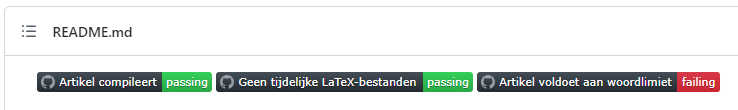
\includegraphics[width=8cm]{figures/iw-badges-voorbeeld.png}
	\caption{GitHub badges}
	\label{fig:badges}
\end{figure}

\flushright{}
Yolande Berbers\\
Gertjan Franken\\
Martijn Sauwens\\
Neline van Ginkel\\
Jan Vermaelen\\
Hans Winderix\\

\end{document}
